\documentclass[a4 paper, 11 pt]{article}

\usepackage[left=0.5in, right=0.5in, top=1in, bottom=1in]{geometry}
\usepackage{fancyhdr}
\usepackage{graphicx}
\usepackage{amsthm}
\usepackage{amsmath}
\usepackage{amssymb}
\usepackage{multirow}
\usepackage{graphicx}

\begin{document}
\begin{titlepage}
\begin{center}
\textsc{\huge Regression Homework 4} \\ [0.5cm]
\textsc{\huge US Home Sales}\\ [1.5cm]
\textsc{\large Janet Ye: jy1151} \\
\vfill
{\large \today}
\end{center}
\end{titlepage}

\section{Introduction}
Number of home sales can be thought of as a demand curve. Basic economic intuition tells us that the demand of home sales is inversely related to the price of homes. In this analysis, we examine the relationship between number of US home sales and several predicting variables, namely, composite housing affordability index, private construction spending, median sales price, unemployment rate, and mortgage rate.
\section{Data}
All data used for this analysis are obtained from St. Louis FRED. The data are not previously seasonably adjusted, and measured on the first of each month ranging from January 1999 to February 2014. We begin by giving a short description about each variable.
\begin{itemize}
\item \textbf{Existing Home Sales}, or the target variable, are based on closing transactions of single-family, townhomes, condominiums and cooperative homes, measured in dollars.
\item \textbf{Housing Affordability Index} measures the degree to which a typical family can afford the monthly mortgage payments on a typical home. Value of 100 means that a family with the median income has exactly enough income to qualify for a mortgage on a median-priced home. An index above 100 signifies that family earning the median income has more than enough income to qualify for a mortgage loan on a median-priced home, assuming a 20 percent down payment. For example, a composite housing affordability index (HAI) of 120.0 means a family earning the median family income has 120\% of the income necessary to qualify for a conventional loan covering 80 percent of a median-priced existing single-family home. An increase in the HAI then shows that this family is more able to afford the median priced home.
\item \textbf{Mortgage Rate} is the 30 year contract interest rates on commitments for fixed-rate first mortgages.
\item \textbf{Construction Spending} is the total private construction spending on residential structures, measured in millions of dollars.
\item \textbf{Median Sales Price, Unemployment Rate} are self-explanatory.
\end{itemize}
Since we are dealing with price, it makes economic sense to use to the log-log model. I logged the response variable -- Existing Home Sales, since it is measured in dollars, as well as ``Construction Spending'' and ``Median Sales Price'', which are both measured in dollars. The other variables, ``Housing Affordability Index'', ``Unemployment'', and ``Mortgage Rate'' stay the same.

Below are scatter plots that show marginal relationship in the data.
\begin{center}
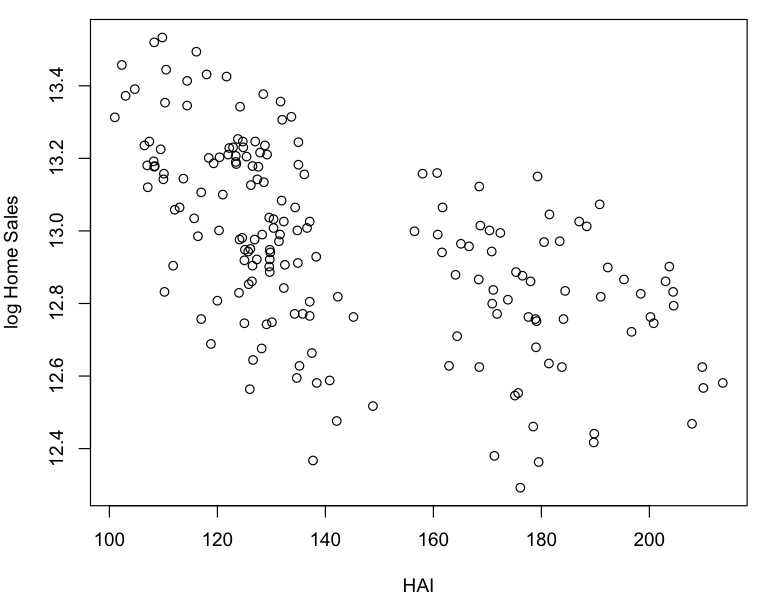
\includegraphics[scale=0.3]{HAI}
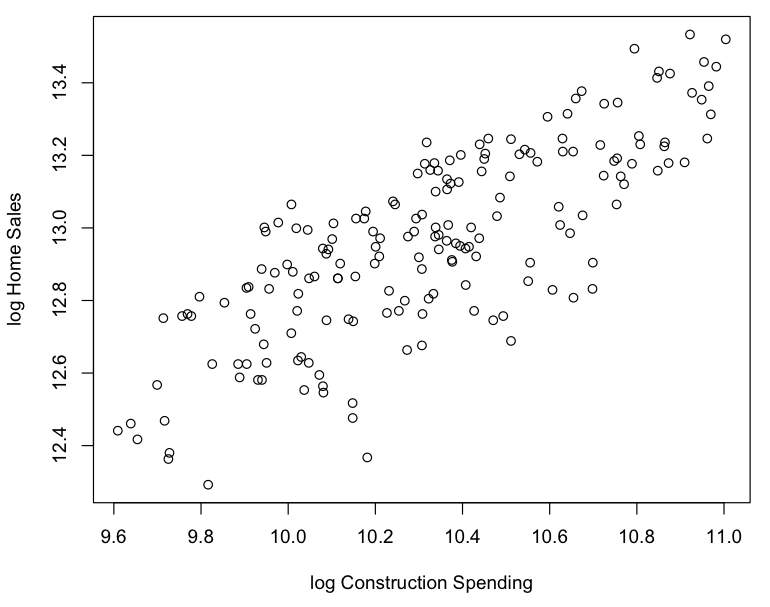
\includegraphics[scale=0.3]{cons}
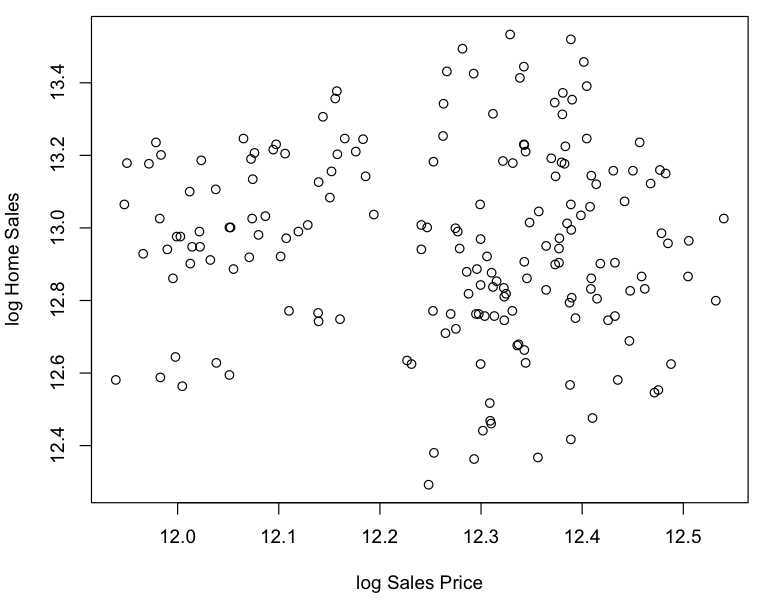
\includegraphics[scale=0.3]{price}
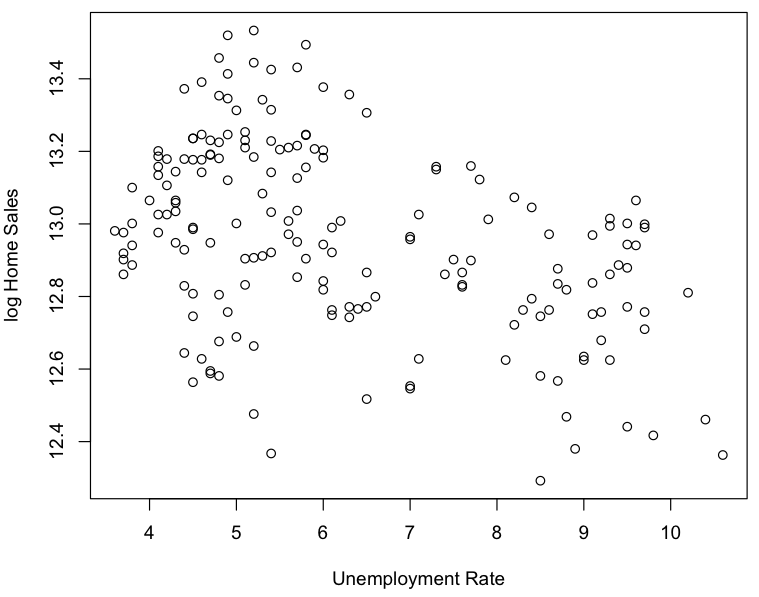
\includegraphics[scale=0.3]{unrate}
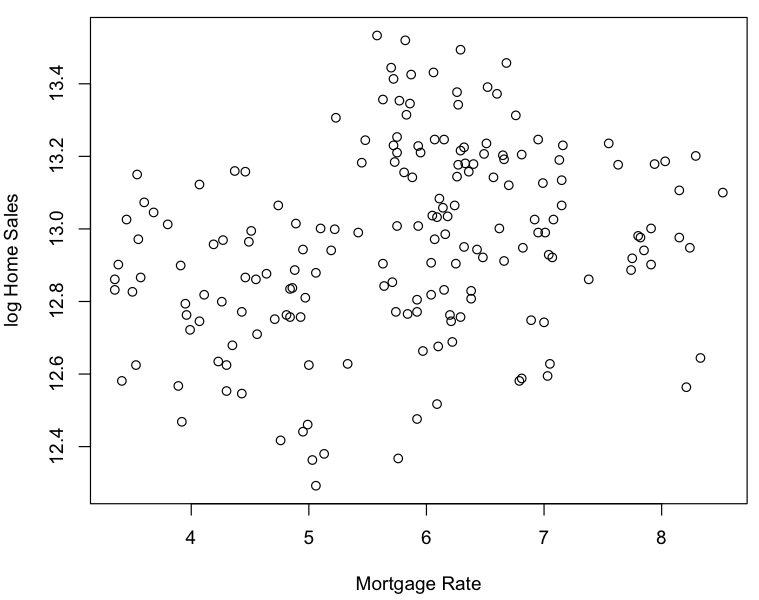
\includegraphics[scale=0.3]{mort}
\end{center}
There is a negative relationship between HAI and log Home Sales, given everything else in the data. One, however, expects this relationship to be positive, as if the more income one has (higher HAI), the more likely one would per chase a house. There also seems to be two subgroups in the data, one clustered below HAI of 140 and the other above 160.

There is a strong, positive, linear marginal relationship between log Construction Spending and log Home Sales. This makes sense: the more money spent on construction is associated with more home sales.

There is no apparent marginal relationship between log Sales Price and log Home Sales. One would expect a negative relationship -- higher sales price is associated with lower home sales.

There is a weak, negative, linear marginal relationship between unemployment rate and log Home Sales. Higher Unemployment Rate is associated with lower Home Sales, which also makes sense.

Lastly, there is no apparent marginal relationship between Mortgage Rate and log Home Sales. One would expect a negative relationship, as higher mortgage rate discourages home sales.

\section{Multiple Regression}
Below is an output of the multiple regression model.
\begin{center}
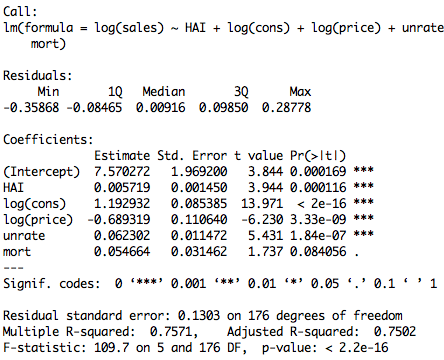
\includegraphics[scale=0.5]{reg} \\
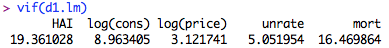
\includegraphics[scale=0.5]{vif}
\end{center}
VIF for both HAI and mortgage are large. Below is a correlation matrix.
\begin{center}
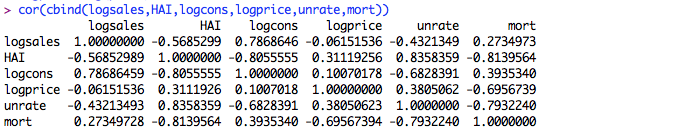
\includegraphics[scale=0.5]{matrix}
\end{center}
HAI has a strong negative correlation (-0.81) with log Construction Spending, a strong positive correlation (0.84) with unemployment rate, a strong negative correlation (-0.81) with mortgage rate.

Besides having a strong negative correlation with mortgage rate as mentioned above, mortgage has a strong negative (-0.79) correlation with unemployment rate.

We proceed to use best subset to determine the best model.
\begin{center}
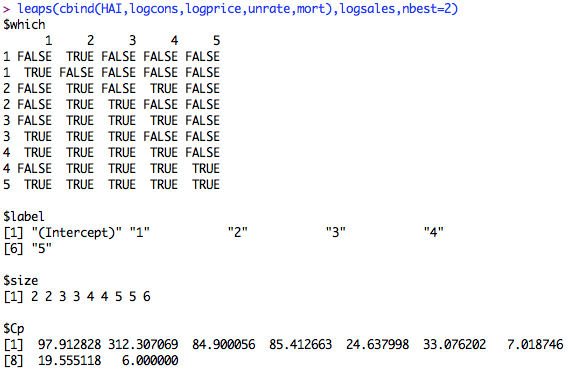
\includegraphics[scale=0.5]{best}
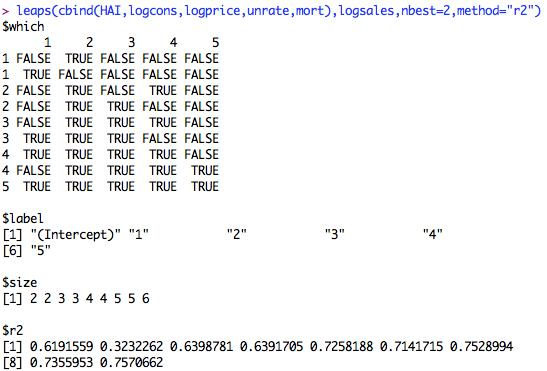
\includegraphics[scale=0.5]{r2}
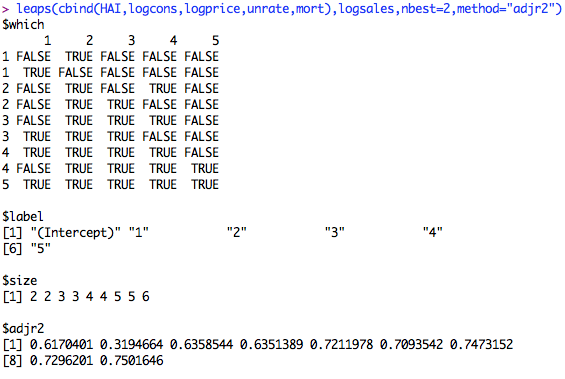
\includegraphics[scale=0.5]{adjr2}
\end{center}
where 1 = HAI, 2 = log construction spending, 3 = log price, 4 = unemployment rate, 5 = mortgage

$R$-squared starts to level off at (value of 0.7528994) for the four-predictor model consisting of HAI, log Construction Spending, log Sales Price, and Unemployment Rate, but $R$-squared is at its highest for the model consisting of all five predictors.
Adjusted $R$-squared is maximized at the five predictor model, a value of 0.75. Another criteria is that $C_p \le p+1 = 5+1 = 6$, where $p$ is number of predictors. The five-predictor model satisfies this condition, with $C_p = 6$. One also wish to minimize $C_p$ value, which is satisfied at the five-predictor model.

Below is output of $AIC$.
\begin{center}
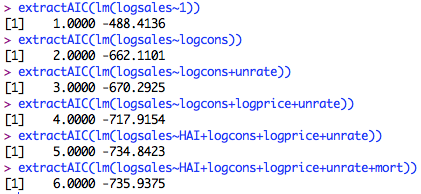
\includegraphics[scale=0.5]{AIC}
\end{center}
$AIC$ is minimized at the five-predictor model, with $AIC$ = -735.9375. We also wish to minimize $AIC_C$. Below are the outputs.
\begin{center}
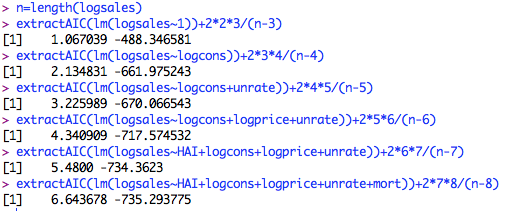
\includegraphics[scale=0.5]{AICC}
\end{center}

$AIC_C$ is minimized for the five-predictor model, at -735.293775. Hence, the five-predictor model is a sensible choice. This is the same multiple regression model as before, and we list the output below again.
\begin{center}
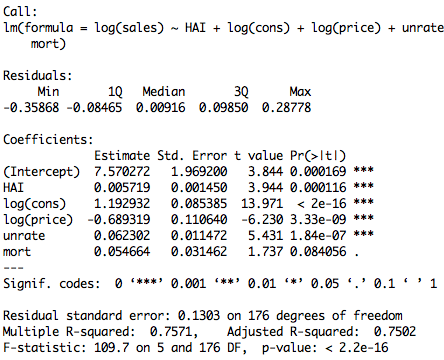
\includegraphics[scale=0.5]{reg}
\end{center}
The regression equation is
\begin{align*}
log \text{ Home Sales} &= 7.570272 + 0.005719 \times \text{HAI} + 1.192932 \times log \text{ Construction Spending} \\
&-0.689319 \times log \text{ Median Sales Price} + 0.062302 \times \text{ Unemployment Rate} \\
&+ 0.054664 \times \text{ Mortgage Rate}
\end{align*}
The intercept is not meaningful at all. One point increase in Housing Affordability Index is associated with 0.57\% increase in home sales, holding all else constant. One percent increase in construction spending is associated with 119.3\% increase in home sales, holding all else constant. One percent increase in median sales price is associated with 69\% decrease in home sales, holding all else constant. One percentage point increase in unemployment rate is associated with 6.23\% increase in Home Sales, holding all else constant. One percentage point increase in mortgage rate is associated with 5.47\% increase in Home Sales, holding all else constant.

The residual standard error implies that our model can predict the response to within a multiplicative factor of 0.5488 to 1.822 $(= 10^{\pm2s})$, 95\% of the time. %fix this

Notice that all predictors but Mortgage are highly significant with small $p$ value for any reasonable $\alpha$. Mortgage has a $p$-value of 0.084, suggesting that the predictor does not add predictive power to the regression.

$R$-squared of 75.71\% means that 75.71\% of the variability in log Home Sales can be explained by the linear relationship with HAI, log Construction Spending, log Median Sales Price, Unemployment Rate, and Mortgage Rate.

\section{Residual Diagnostics}
\begin{center}
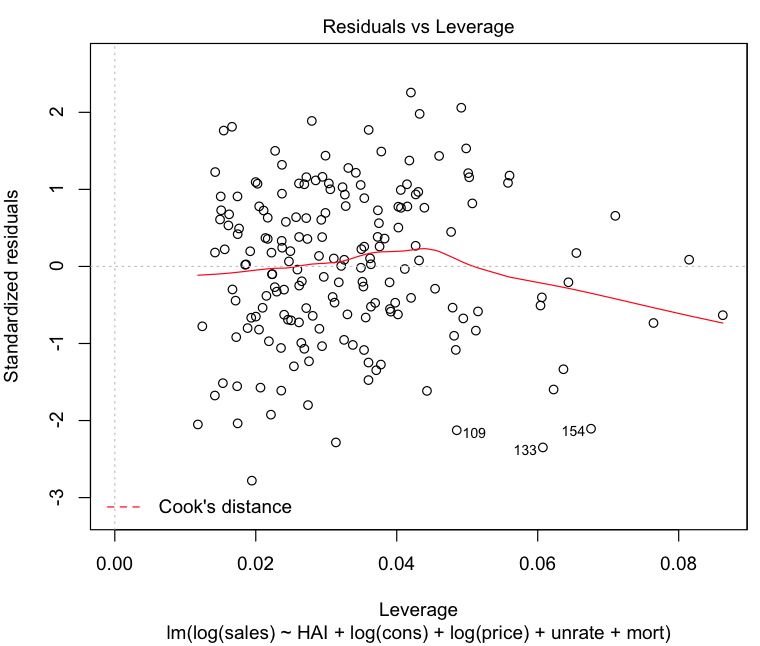
\includegraphics[scale=0.4]{diag}
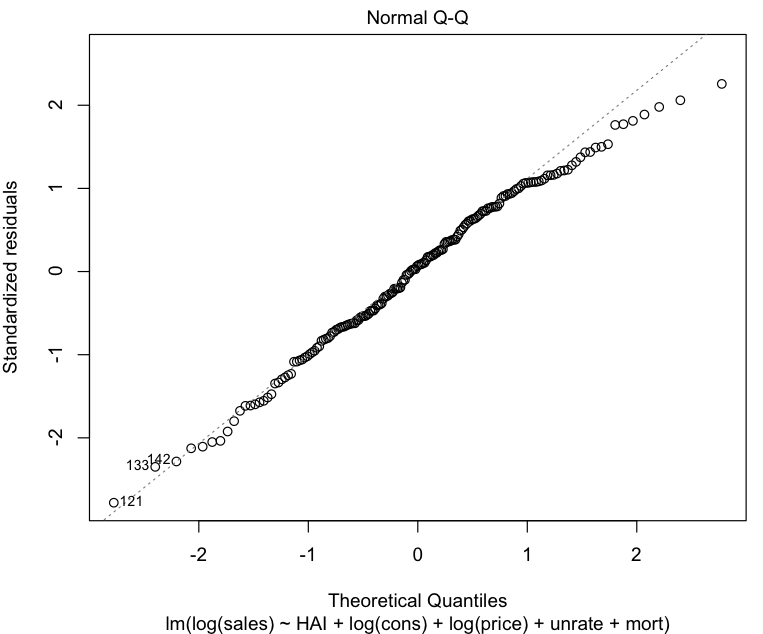
\includegraphics[scale=0.4]{QQ}
\end{center}
Most residuals are within $\pm 2.5$ standardized deviation. A good guideline for leverage value is $2.5 \left(\frac{5+1}{182}\right) = 0.0824$. Almost all points satisfy this criteria. $R$ marks two bands in red dotted lines. The lines are not shown in this plot using the scale shown, meaning that the points very well satisfy Cook's D $<1$.

There is a trail of points below the line on the far right. This suggests that the data is probably skewed right.%add 

Here is a plot of standardized residual versus time plot.
\begin{center}
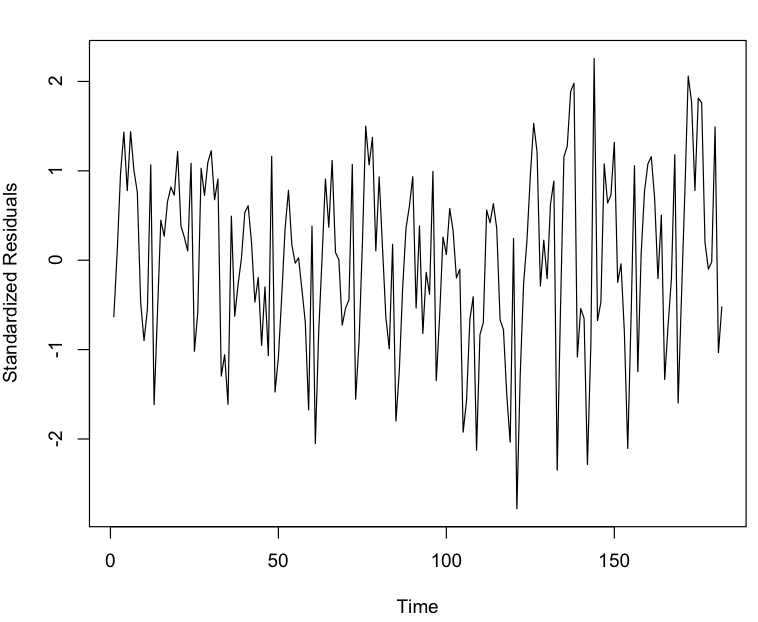
\includegraphics[scale=0.4]{time}
\end{center}
Autocorrelation is apparent. In fact, Durbin-Watson Test agrees.
\begin{center}
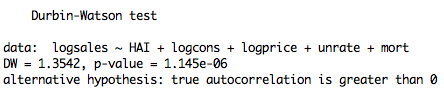
\includegraphics[scale=0.5]{DW}
\end{center}
We have 182 data points. $DW = 1.3542$, which is highly significant. $R$ gives a $p$-value of almost zero, showing that there is a sign of positive autocorrelation.

Below is an $ACF$ plot of the standardized residuals, checking if observed autocorrelations appear to be consistent with the $AR(1)$ model.
\begin{center}
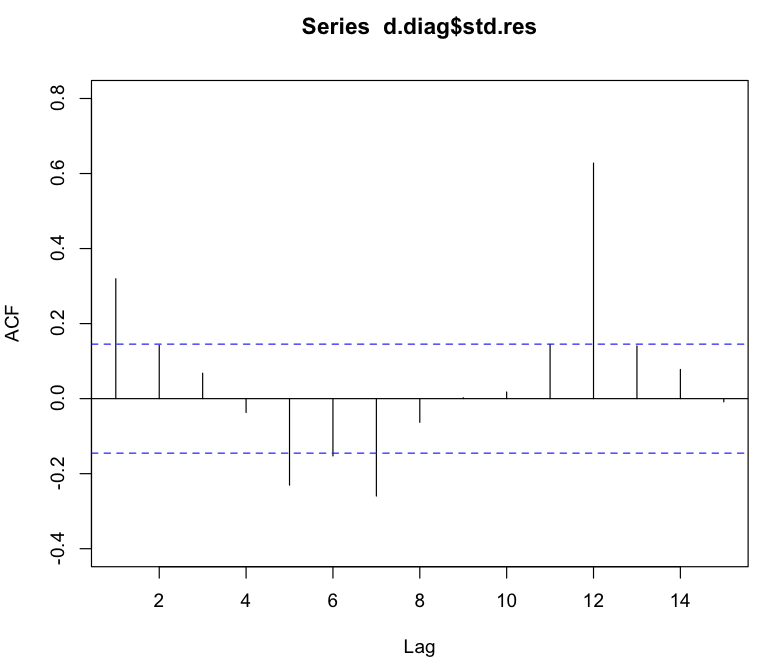
\includegraphics[scale=0.4]{ACF} 
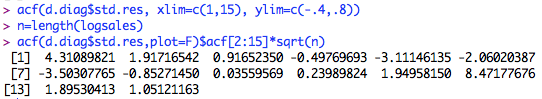
\includegraphics[scale=0.5]{ACFz}
\end{center}
Note that the autocorrelations decay roughly at the geometric rate consistent with an $AR(1)$ process, supporting the Durbin-Watson test. The first lag is significantly different from zero, with a $z-$statistics of 4.31. Notice that the twelfth lag spikes, and has a $z$-statistics of 8.47, which is highly significant. This shows there is autocorrelation, since we have monthly data, and lags spike at multiples of 12.

The Runs Test is also significant.
\begin{center}
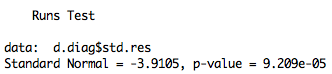
\includegraphics[scale=0.6]{runs}
\end{center}
$R$ gives a $p$-value of $9.209 \times 10^{-5}$, which is below any reasonable $\alpha$. All three methods suggest autocorrelation.

\section{Addressing Autocorrelation}
From $ACF$ plot, we see a seasonable effect, i.e. lag 12. We can then include seasonal indicator variables as additional predictors in the regression model.
\begin{center}
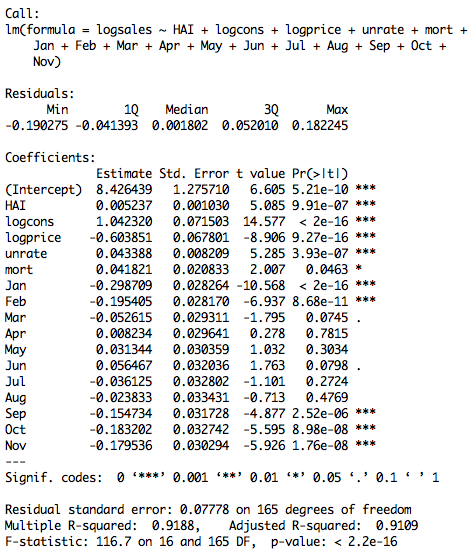
\includegraphics[scale=0.5]{reg2} \\
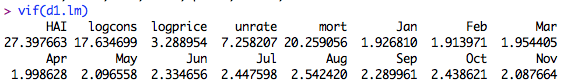
\includegraphics[scale=0.5]{vif2}
\end{center}
This model is strong, with $R$-squared of 91.88\%. However, $VIF$ is high for HAI, log Construction Spending, and Mortgage Rate. $t$-statistics for Mar, Apr, May, Jun, Jul, and Aug are not statistics with $p$-value greater than 0.05. It makes sense to include all eleven indicator variables. Nonetheless, the best subset tests are included below.

We proceed with best subset test, where 1 = HAI, 2 = log Construction Spending, 3 = log Sales Price, 4 = Unemployment Rate, 5 = Mortgage Rate, 6 = Jan, 7 = Feb, 8 = Mar, 9 = Apr, A = May, B = Jun, C = Jul, D = Aug, E = Sep, F = Oct, G = Nov.
\begin{center}
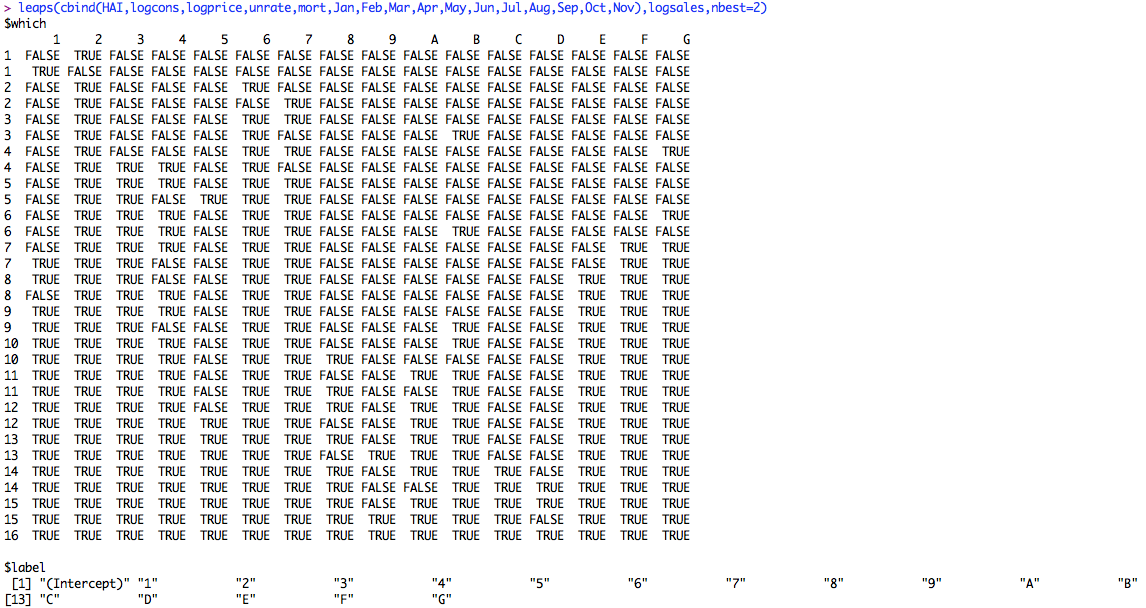
\includegraphics[scale=0.5]{best2a}
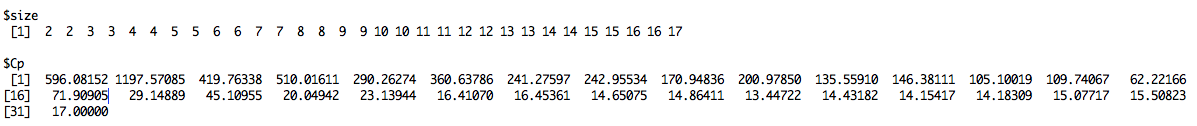
\includegraphics[scale=0.4]{best2b}
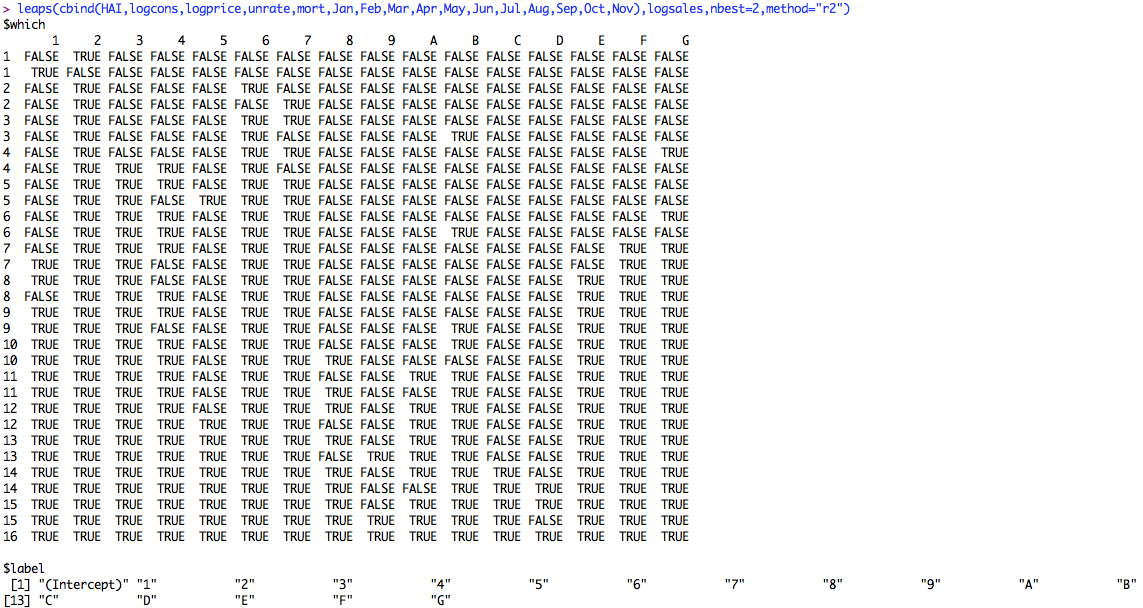
\includegraphics[scale=0.5]{r2a}
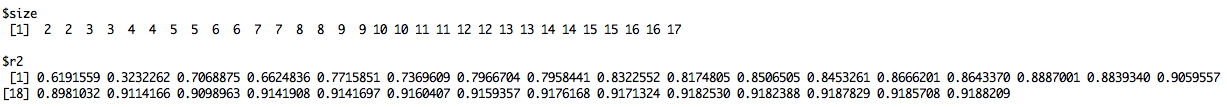
\includegraphics[scale=0.4]{r2b}
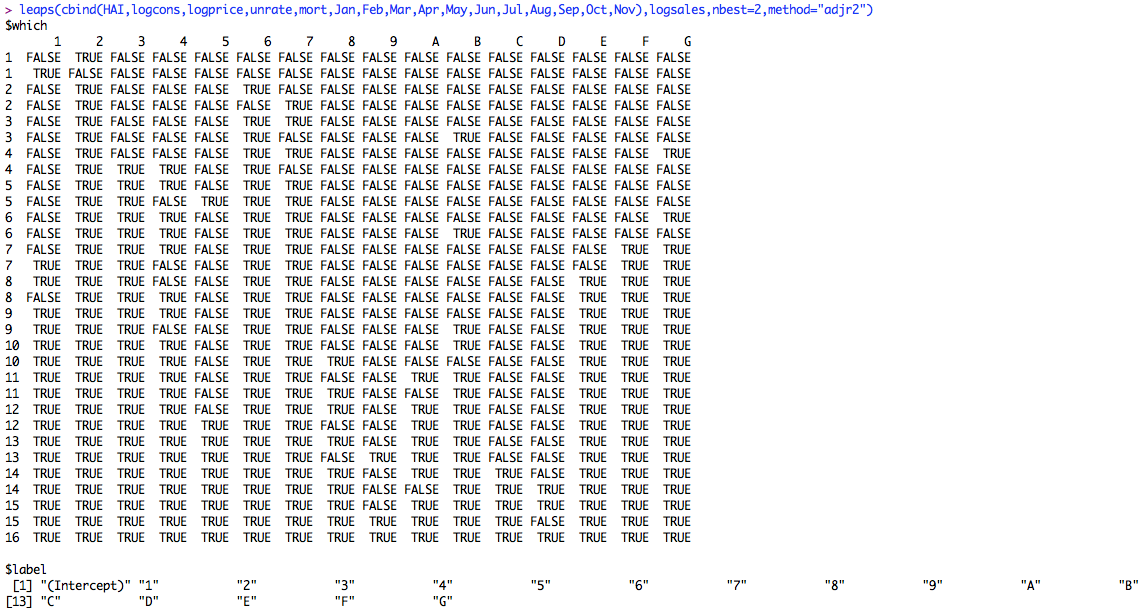
\includegraphics[scale=0.5]{adjr2a}
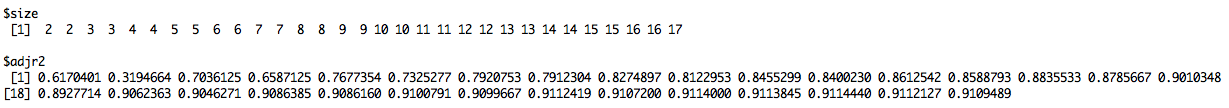
\includegraphics[scale=0.4]{adjr2b}
\end{center}
$R$-squared begins to level off (91.14\%) at 10-predictor model consisting HAI, log Construction Spending, log Sales Price, Unemployment Rate, Jan, Feb, Jun, Sep, Oct, and Nov. Adjusted $R$-squared is maximized (91.14\%) at 14-predictor model, with all predictors except Apr and Aug. We want $C_p \le p+1 = 16+1 = 17$, which is realized at 11-predictor model, with predictors HAI, log Construction Spending, log Sales Price, Unemployment Rate, Jan, Feb, May, Jun, Sep, Oct, and Nov. $C_p$ is minimized at the 13-predictor model, with all predictors except Apr, Jul, and Aug.
\begin{center}
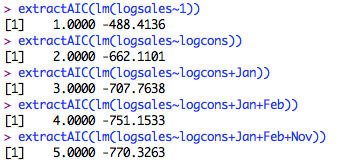
\includegraphics[scale=0.4]{AIC1}\\
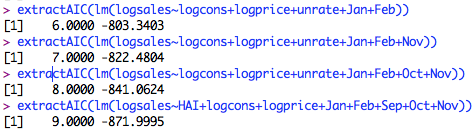
\includegraphics[scale=0.4]{AIC2}\\
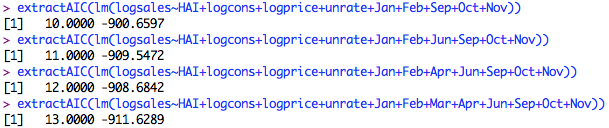
\includegraphics[scale=0.4]{AIC3}\\
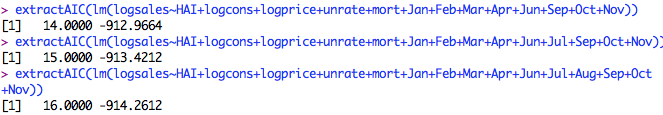
\includegraphics[scale=0.4]{AIC4}\\
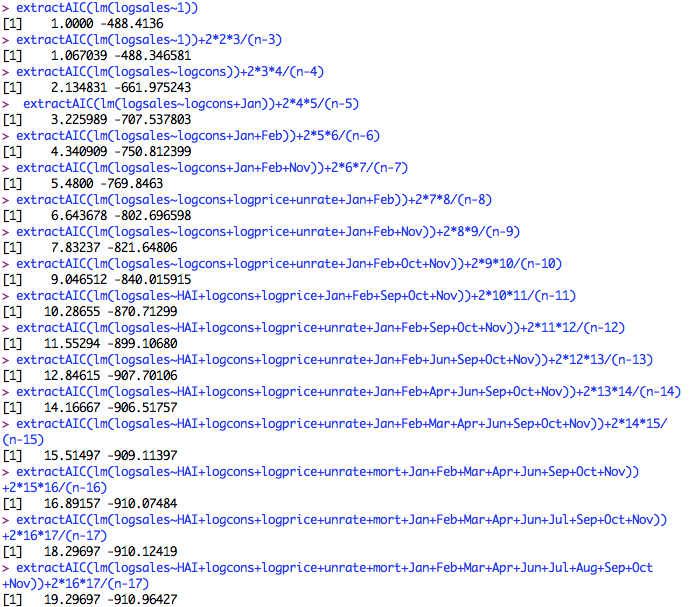
\includegraphics[scale=0.4]{AICC2}
\end{center}
Both $AIC$ and $AIC_C$ are minimized using all  predictors. If we choose to use all variables, autocorrelation is still noticeable in the following standardized error versus time plot, despite the fact that we included indicator variables.
\begin{center}
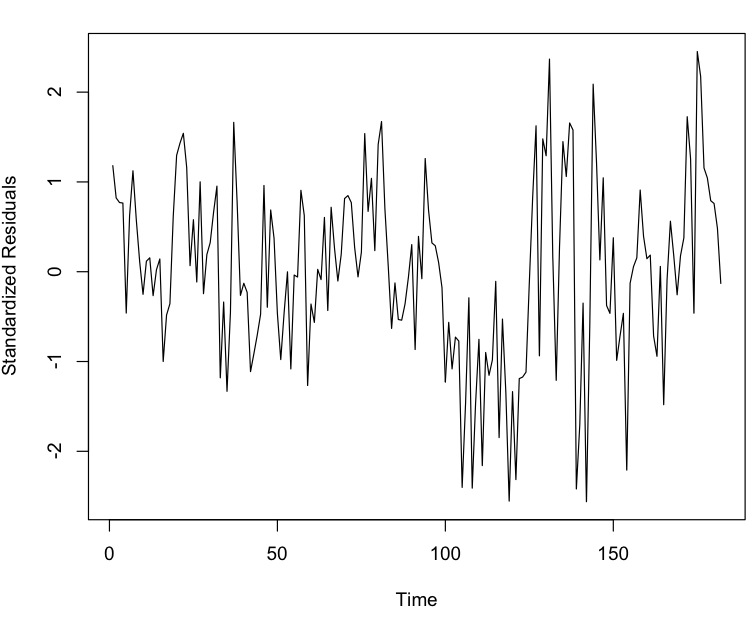
\includegraphics[scale=0.4]{all}
\end{center}
Instead, we can choose to include lagged variables for log Construction Spending, Unemployment Rate, Mortgage, log Sales Price, log Home Sales. Below are some scatterplots, showing logsales versus each of the new variable created.

\begin{center}
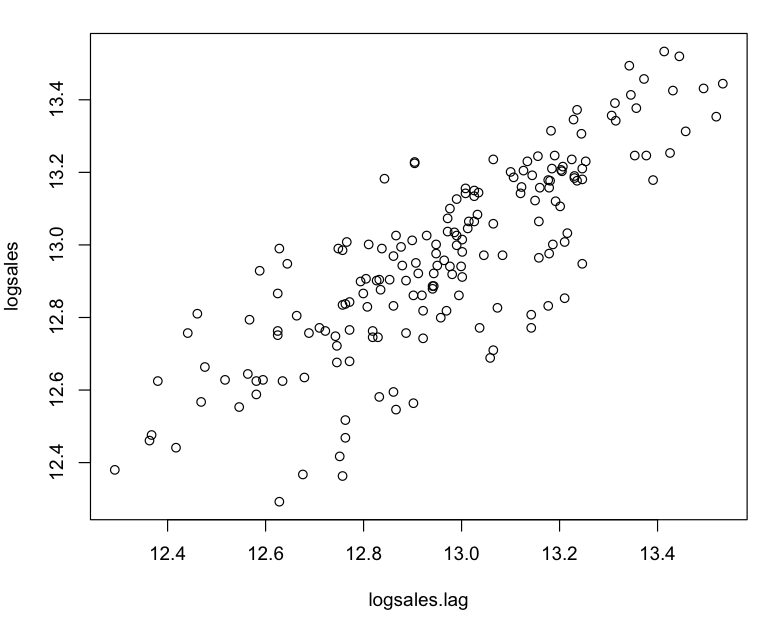
\includegraphics[scale=0.3]{salessales}
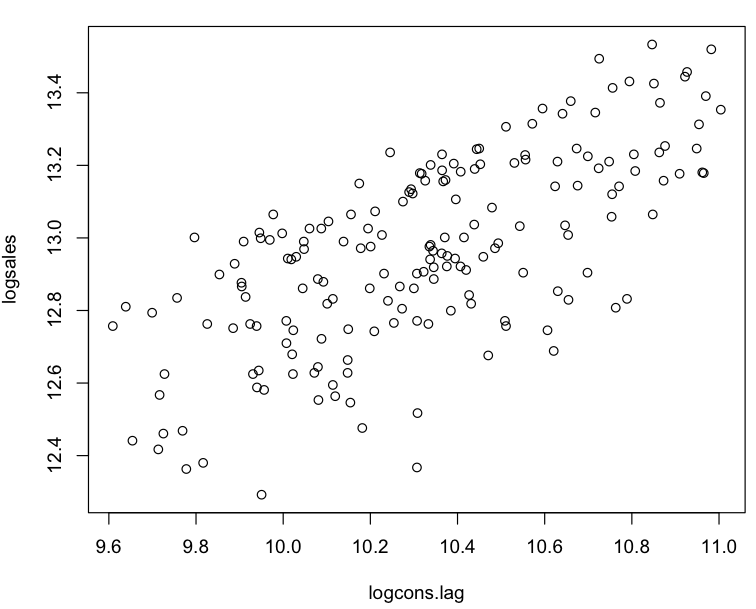
\includegraphics[scale=0.3]{salescons}
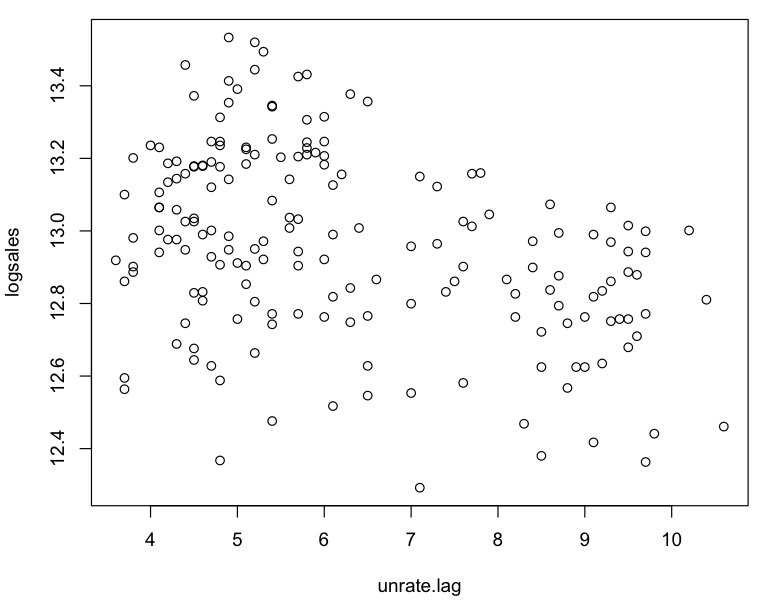
\includegraphics[scale=0.3]{salesunrate}
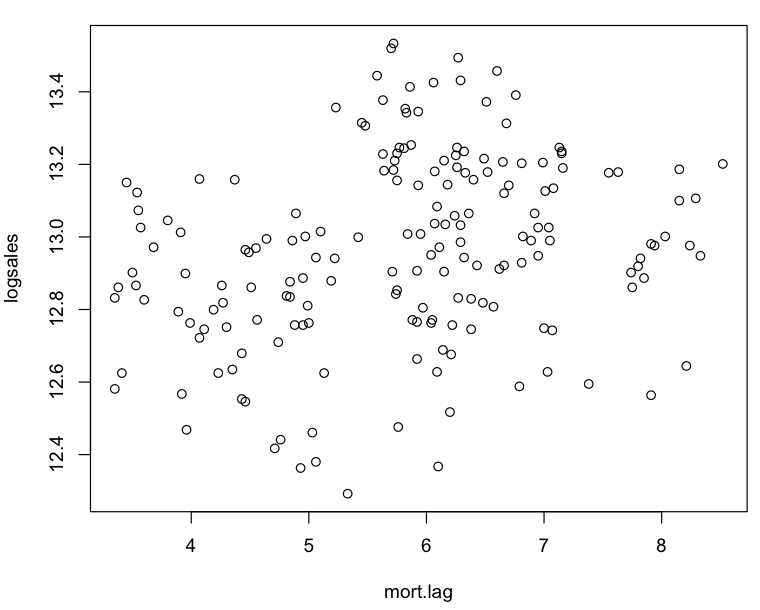
\includegraphics[scale=0.3]{salesmort}
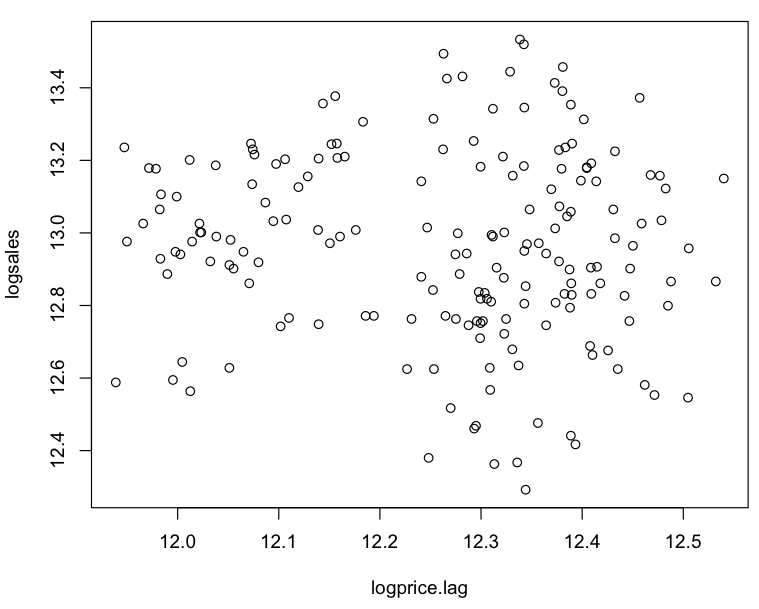
\includegraphics[scale=0.3]{salesprice}
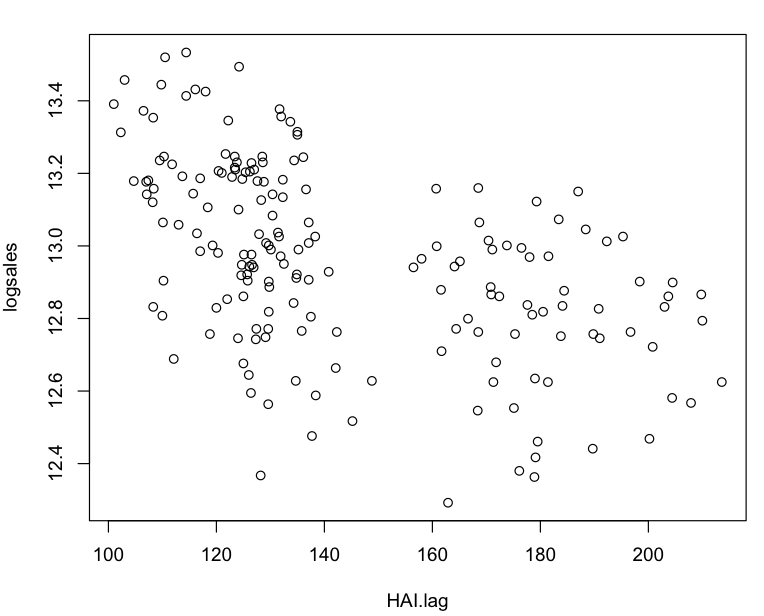
\includegraphics[scale=0.3]{saleshai}
\end{center}
The marginal relationships between log sales versus each of lagged unemployment rate, lagged mortgage, and lagged log sales price are not clear. Again, there seems to be subgroups in logsales versus lagged HAI plot. Other relationships are fairly strong.

Since from previously, we see that every January has a peak in home sales, we also include a indicator variable for January.

Below is the regression.
\begin{center}
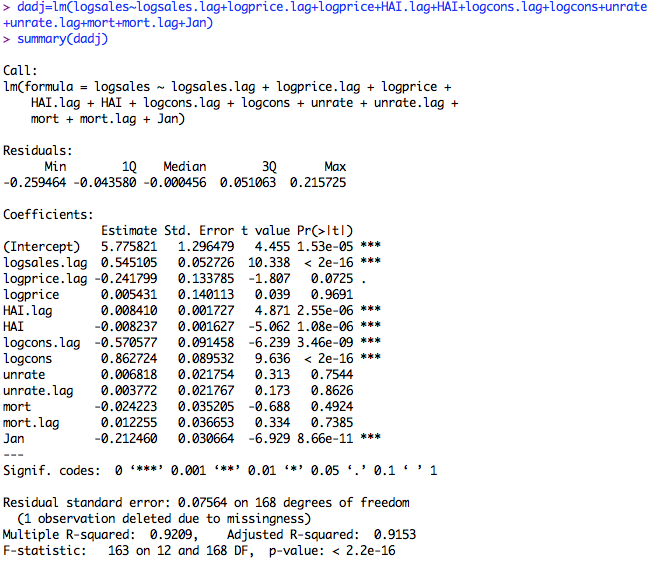
\includegraphics[scale=0.4]{d3lm}\\
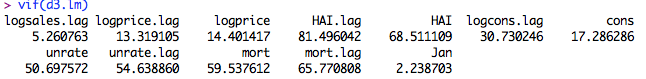
\includegraphics[scale=0.4]{d3vif}
\end{center}
There are signs of multicollinearity between variable and lagged variables, but that is expected. The model is fairly strong with $R$-squared of 91.25\%. \begin{center}
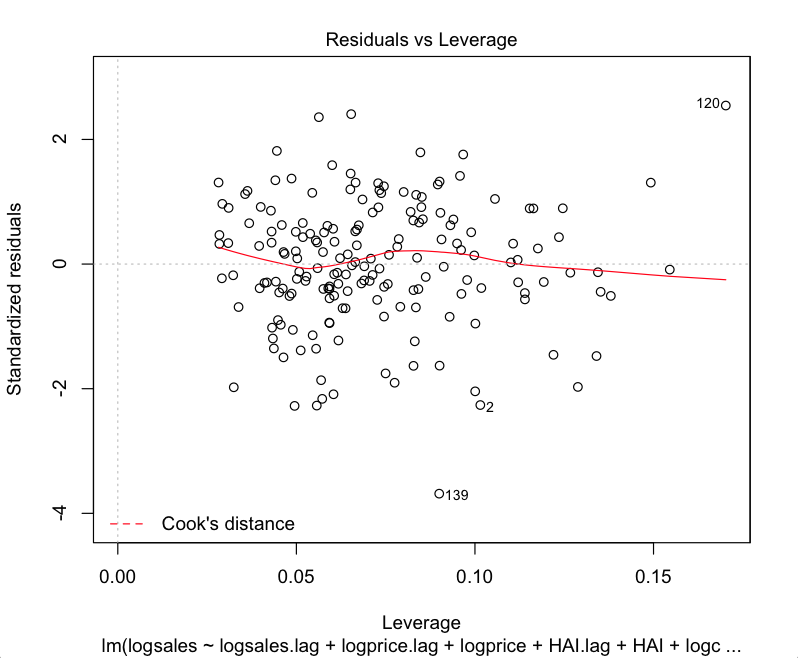
\includegraphics[scale=0.4]{d3diag}
\end{center}
A quick regression diagnostic shows that standardized residuals are fairly randomly scatter and within $\pm 2.5$. There are two potential outliers, observation 120 and 139. Observation 120 is December 2008 and observation 139 is July 2010. Below show part of the data that con taints the two outliers.

\begin{center}
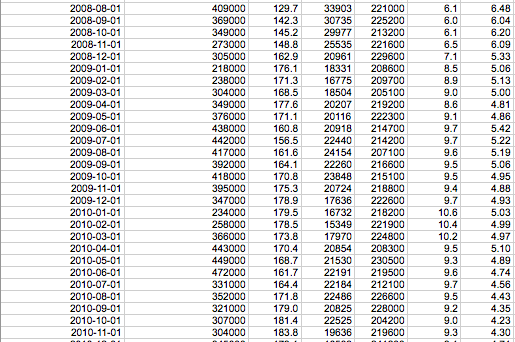
\includegraphics[scale=0.6]{outlier}
\end{center}

The second column represents home sales. Notice in December 2008, home sales is 305000 units, but in January 2009, it dips to 218000 units. In July 2010, home sales decreased to 331000 units from 472000 from previous month. The dip in December 2008 might be from the financial crisis. While July 2010 is indeed another unusual point.

A good guideline for the leverage value is $2.5\left(\frac{12+1}{182}\right) = 0.17$. All points satisfy this criteria. Cook's distance is also fine, for reason mentioned previously. We ignore the two outliers for now.

We then look at autocorrelation.
\begin{center}
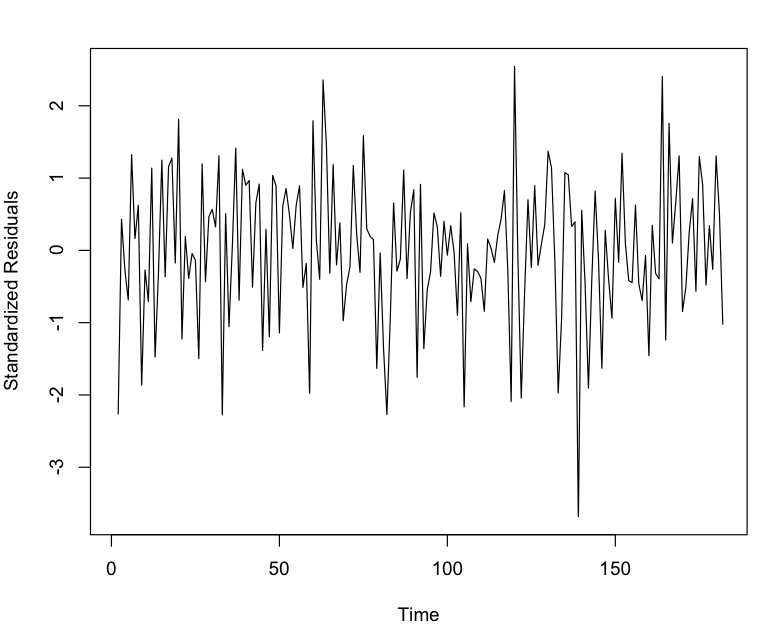
\includegraphics[scale=0.3]{d3time}
\end{center}
There is still signs of autocorrelation in the standardized residual versus time plot. 
\begin{center}
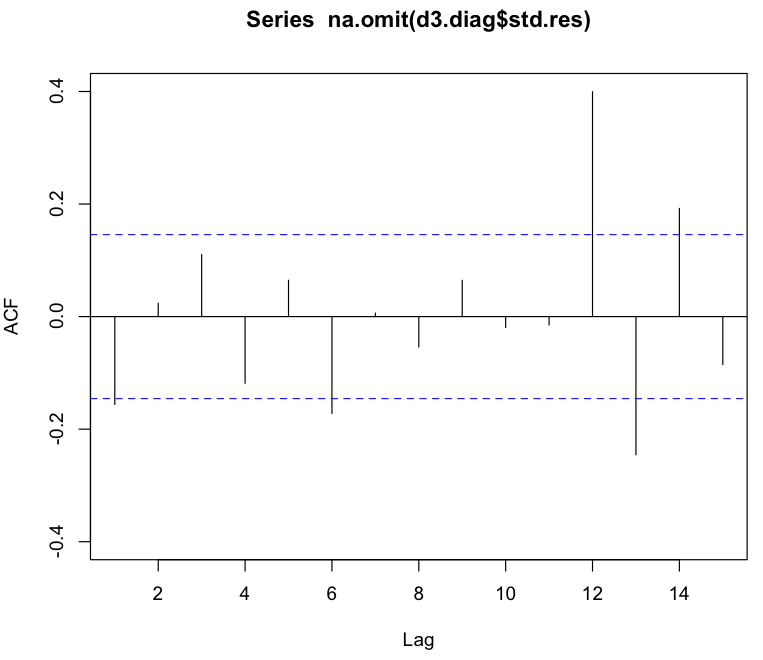
\includegraphics[scale=0.3]{d3acf} \\
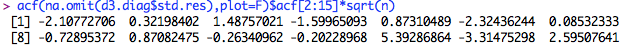
\includegraphics[scale=0.4]{d3acfz} \\
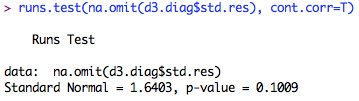
\includegraphics[scale=0.4]{d3runs}
\end{center}
The first lag in $ACF$ plot is still slightly significant. The twelfth lag is still not fixed. However, runs test is not significant anymore, we have $p$-value of -0.1. \textit{[How to obtain DW test for data with lagged variables? Gasoline Price does not include this part of $R$ code]}

\section{Outliers}
We may address the outliers by assigning average of the periods immediately preceding and succeeding the outliers. Regression output is shown below.
\begin{center}
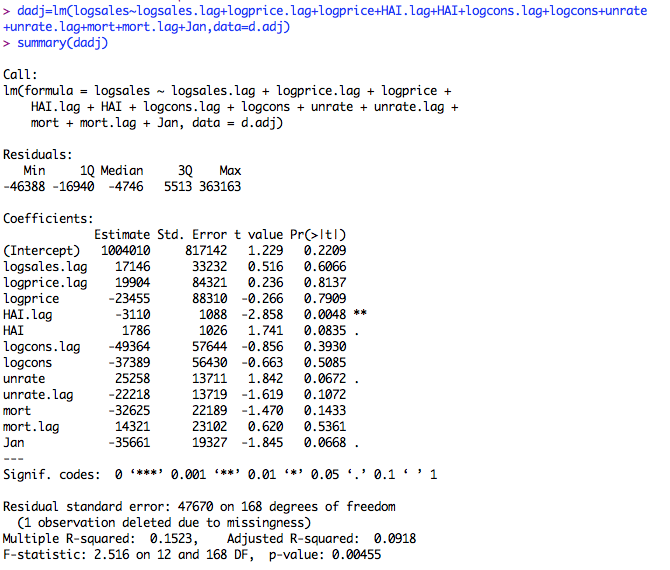
\includegraphics[scale=0.4]{flm}
\includegraphics[scale=0.5]{fvif}
\includegraphics[scale=0.4]{fqq}
\includegraphics[scale=0.4]{fsd}
\end{center}
Noticing after adjusting the points, $R$-squared dropped to 15\%. The standardized residuals are unbelievably high (roughly 8) for observation 139 and observation 140. The standardized residuals is roughly 4 for observation 120. It is obvious that we fail to address the issue of outlier. The QQ plot now sees observation 121 as an outlier. Adjusting observation 139 now makes observation 140 influential. At this point, the basic method does not seem to address the issue of outliers. Our regression seems to fail.
\section{Remarks}
The model is built using data that are not seasonably adjusted. Thus we run into many problems. The Fed, however, does post seasonally adjusted data, for variables such as unemployment rate and mortgage rate. I was unable to obtain seasonally adjusted mortgage rate, adjusted HAI, and adjusted construction spending, whence unable to produce a multiple regression using adjusted data. The adjusted data are usually reported in deseasonalized form, which roughly corresponds to taking the residuals from a regression on the monthly effects and adding the overall average data back.

Despite the unsuccessful attempt to remove the outliers, our model still offers some insight.
\end{document}
%home sales ~ housing affordability index + private construction spending + median sales price + unemployment + mortgage rate